\chapter{Results} % Main chapter title

\label{Chapter7} % For referencing this chapter elsewhere, use \ref{Chapter7}

\lhead{Chapter 7. \emph{Results}}

%----------------------------------------------------------------------------------------
%	SECTION 7.1 - Results
%----------------------------------------------------------------------------------------

\section{Results}

%----------------------------------------------------------------------------------------
%	SUBSECTION 7.1.1 - Results Graphs
%----------------------------------------------------------------------------------------

\subsection{Results Graphs}

This section will present several graphs taken from data extracted throughout the experiments. First of all, precisions are needed on the experiments themselves. \emph{Brevitas} is still in development and several functionalities are still missing. While the main idea was to use several well-known network architectures (\emph{LeNet-5}, \emph{AlexNet}, \emph{VGG}, and \emph{Mobilenet}), the reality is that most of these networks are not yet supported by the export functionality. This export is crucial as it allows one to port its \emph{Brevitas}-defined and trained network and export it to \emph{ONNX} before importing it in \emph{FINN} and deploying it on an FPGA.

In the end, out of the three networks presented in the last chapter, only the \emph{TFC} network can make the full run, through training, export and on FPGA. The \emph{CNV} network gets stuck through several transformations and sequence of layers that are not yet supported by the streamlining process. On the other hand, \emph{MobilenetV1} is not even exporting to \emph{ONNX} and was chosen to be stopped.

However, \emph{TFC} training results can be seen on \emph{Figure} \ref{fig:TFCErrorRate} where the different configuration A\emph{X}W\emph{X}, where \emph{X} is the bitwidth of both activations and weights. The different configurations have been trained for 40 epochs in total and a model has been kept for evaluation every 10 epochs. The graph represents the error rate (or $100 - accuracy$) given the training time.

% GRAPH ACCURACY TRAINING TIME TFC
\begin{figure}[htbp]
\centering
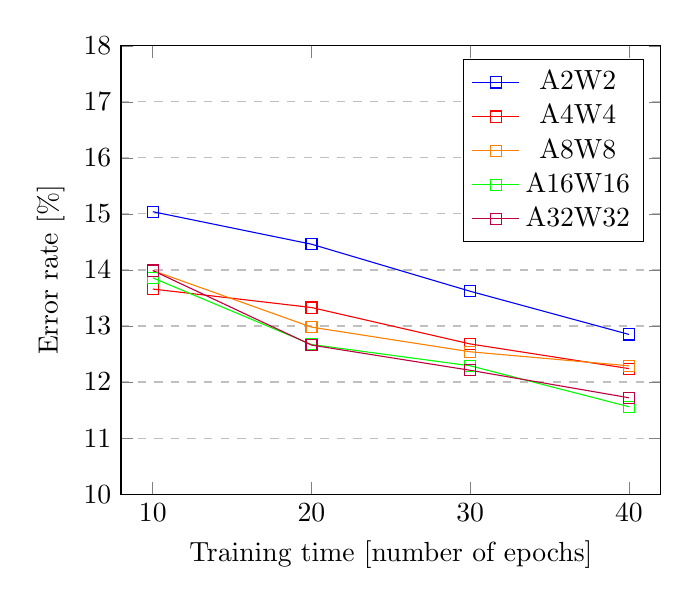
\begin{tikzpicture}
\begin{axis}[
    xlabel={Training time [number of epochs]},
    ylabel={Error rate [\%]},
    xmin=8, xmax=42,
    ymin=10, ymax=18,
    xtick={0,10,20,30,40},
    ytick={10,11,12,13,14,15,16,17,18},
    legend pos=north east,
    ymajorgrids=true,
    grid style=dashed,
]
% TFC A2W2:   84.960 | 85.540 | 86.380 | 87.150
\addplot[
    color=blue,
    mark=square,
    ]
    coordinates {
    (10,15.04)(20,14.46)(30,13.62)(40,12.85)
    };
% TFC A4W4:   86.340 | 86.670 | 87.320 | 87.760
\addplot[
    color=red,
    mark=square,
    ]
    coordinates {
    (10,13.66)(20,13.33)(30,12.68)(40,12.24)
    };
% TFC A8W8:   86.010 | 87.020 | 87.460 | 87.710
\addplot[
    color=orange,
    mark=square,
    ]
    coordinates {
    (10,13.99)(20,12.98)(30,12.54)(40,12.29)
    };
% TFC A16W16: 86.140 | 87.330 | 87.710 | 88.440
\addplot[
    color=green,
    mark=square,
    ]
    coordinates {
    (10,13.86)(20,12.67)(30,12.29)(40,11.56)
    };
% TFC A32W32: 86.010 | 87.340 | 87.690 | 88.280
\addplot[
    color=purple,
    mark=square,
    ]
    coordinates {
    (10,13.99)(20,12.66)(30,12.21)(40,11.72)
    };
\legend{A2W2,A4W4,A8W8,A16W16,A32W32}
\end{axis}
\end{tikzpicture}
\caption[TFC Error Rate]{TFC error rate against training time}
  \label{fig:TFCErrorRate}
\end{figure}

While the \emph{CNV} network could not be deployed, it could still be trained and the results can be seen on \emph{Figure} \ref{fig:CNVErrorRate}. As in the \emph{TNC} figure, the configurations are named A\emph{X}W\emph{X}, where \emph{X} is the bitwidth.

% GRAPH ACCURACY TRAINING TIME CNV
\begin{figure}[htbp]
\centering
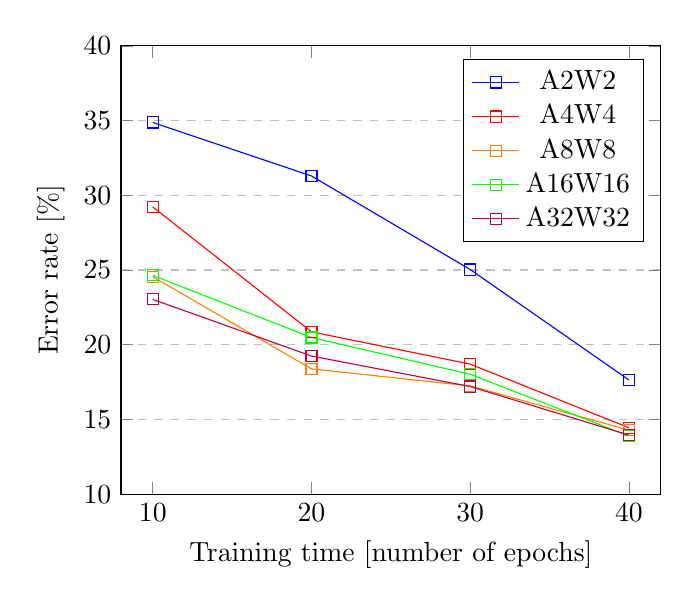
\begin{tikzpicture}
\begin{axis}[
    xlabel={Training time [number of epochs]},
    ylabel={Error rate [\%]},
    xmin=8, xmax=42,
    ymin=10, ymax=40,
    xtick={0,10,20,30,40},
    ytick={10,15,20,25,30,35,40},
    legend pos=north east,
    ymajorgrids=true,
    grid style=dashed,
]
% CNV A2W2:   65.130 | 68.710 | 76.970 | 82.360
\addplot[
    color=blue,
    mark=square,
    ]
    coordinates {
    (10,34.87)(20,31.29)(30,25.03)(40,17.64)
    };
% CNV A4W4:   70.780 | 79.140 | 81.300 | 85.560
\addplot[
    color=red,
    mark=square,
    ]
    coordinates {
    (10,29.22)(20,20.86)(30,18.70)(40,14.44)
    };
% CNV A8W8: 75.450 | 81.620 | 82.760 | 85.720
\addplot[
    color=orange,
    mark=square,
    ]
    coordinates {
    (10,24.55)(20,18.38)(30,17.24)(40,14.28)
    };
% CNV A16W16: 75.360 | 79.520 | 81.980 | 86.110
\addplot[
    color=green,
    mark=square,
    ]
    coordinates {
    (10,24.64)(20,20.48)(30,18.02)(40,13.89)
    };
% CNV A32W32: 72.970 | 80.760 | 82.800 | 86.050
\addplot[
    color=purple,
    mark=square,
    ]
    coordinates {
    (10,23.03)(20,19.24)(30,17.20)(40,13.95)
    };

\legend{A2W2,A4W4,A8W8,A16W16,A32W32}
\end{axis}
\end{tikzpicture}
\caption[CNV Error Rate]{CNV error rate against training time}
  \label{fig:CNVErrorRate}
\end{figure}

Both graphs show a separation in three sections: 2-bits precision, 4- and 8-bits precision and 16- and 32-bits precision. This separation is seen in terms of reaction to the training. For the \emph{TFC} network, the result of the training, after 40 epochs shows three separate points: $\sim$13\% error rate for A2W2, $\sim$12.3\% error rate for A4W4 and A8W8 and $\sim$11.6\% for A16E16 and A32W32. On the other hand for the \emph{CNV} network, there is a clear separation between A2W2 at $\sim$17.5\% and all the other configurations at $\sim$14.8%

Now if we look deeper into the \emph{TFC} deployment, we can get other important metrics from the experiments. First, \emph{Figure} \ref{fig:TFCThroughput} shows the throughput compared to the error rate determined earlier. Note that the error rate for a 40-epochs long training is used.

The three metrics presented in the next graphs are: \emph{throughput}, the number of images the deployed network can process in one second ; \emph{DRAM in bandwidth}, the amount of data that can be processed coming from the DRAM in to the FPGA board ; \emph{DRAM out banwidth}, the amount of data that can be processed coming from the FPGA board out to the DRAM.

\begin{itemize}
  \item \textbf{Throughput}(\emph{Figure} \ref{fig:TFCThroughput}): If the throughput seems nearly identical for A2W2 and A4W4, going to A8W8 makes one lose more than 10 thousands images per second. And even worse, using A16W16 consists of a loss of over 45 thousands images per second.

  % THROUGHPUT FIGURE
  \begin{figure}[htbp]
  \centering
  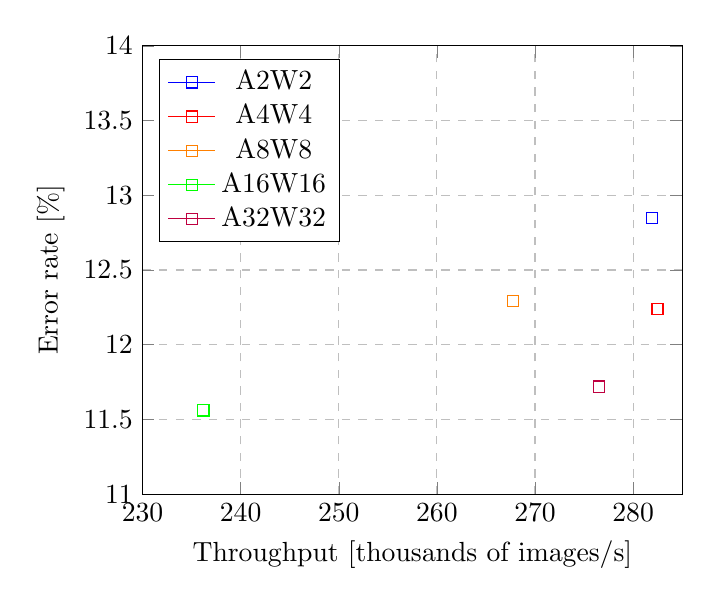
\begin{tikzpicture}
  \begin{axis}[
    xlabel={Throughput [thousands of images/s]},
    ylabel={Error rate [\%]},
    xmin=230, xmax=285,
    ymin=11, ymax=14,
    xtick={230,240,250,260,270,280},
    ytick={11,11.5,12,12.5,13,13.5,14},
    legend pos=north west,
    ymajorgrids=true,
    xmajorgrids=true,
    grid style=dashed,
    ]
  % A2W2
  \addplot+ [
      color=blue,
      mark=square
      ] coordinates {(281.951,12.85)};
  % A4W4
  \addplot+ [
      color=red,
      mark=square
      ] coordinates {(282.483,12.24)};
  % A8W8
  \addplot+ [
      color=orange,
      mark=square
      ] coordinates {(267.732,12.29)};
  % A16W16
  \addplot+ [
      color=green,
      mark=square
      ] coordinates {(236.205,11.56)};
  % A32W32
  \addplot+ [
      color=purple,
      mark=square
      ] coordinates {(276.541,11.72)};
  \legend{A2W2,A4W4,A8W8,A16W16,A32W32}
  \end{axis}
  \end{tikzpicture}
  \caption[TFC Throughput]{TFC error rate compared to throughput}
    \label{fig:TFCThroughput}
  \end{figure}


  \item \textbf{DRAM in bandwidth}(\emph{Figure} \ref{fig:TFCDRAMIn}): The same conclusions can be used for the DRAM bandwidth. The more the bitwidth, the lower the bandwidth, with an exception fo A4W4 that outperforms A2W2 being at 288 against 283 Mb/s.

  % DRAM in bandwidth FIGURE
  \begin{figure}[htbp]
  \centering
  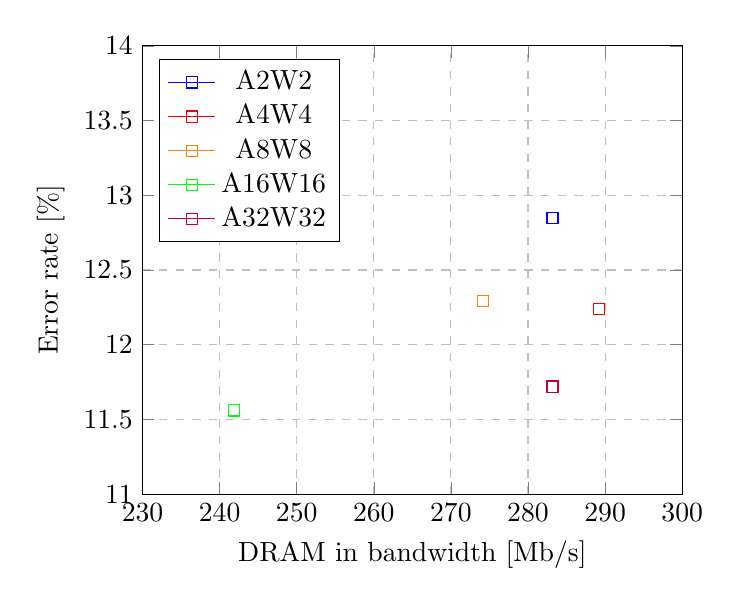
\begin{tikzpicture}
  \begin{axis}[
    xlabel={DRAM in bandwidth [Mb/s]},
    ylabel={Error rate [\%]},
    xmin=230, xmax=300,
    ymin=11, ymax=14,
    xtick={230,240,250,260,270,280,290,300},
    ytick={11,11.5,12,12.5,13,13.5,14},
    legend pos=north west,
    ymajorgrids=true,
    xmajorgrids=true,
    grid style=dashed,
    ]
  % A2W2
  \addplot+ [
      color=blue,
      mark=square
      ] coordinates {(283.18,12.85)};
  % A4W4
  \addplot+ [
      color=red,
      mark=square
      ] coordinates {(289.26,12.24)};
  % A8W8
  \addplot+ [
      color=orange,
      mark=square
      ] coordinates {(274.16,12.29)};
  % A16W16
  \addplot+ [
      color=green,
      mark=square
      ] coordinates {(241.87,11.56)};
  % A32W32
  \addplot+ [
      color=purple,
      mark=square
      ] coordinates {(283.18,11.72)};
  \legend{A2W2,A4W4,A8W8,A16W16,A32W32}
  \end{axis}
  \end{tikzpicture}
  \caption[TFC DRAM in]{TFC DRAM in bandwidth when compared to error rate}
    \label{fig:TFCDRAMIn}
  \end{figure}

  \item \textbf{DRAM out bandwidth}(\emph{Figure} \ref{fig:TFCDRAMOut}): While the graph presents the same impressions as the DRAM in, the results for A2W2 and A4W4 are this time nearly identical around 11.3Mb/s


  % DRAM out bandwidth FIGURE
  \begin{figure}[htbp]
  \centering
  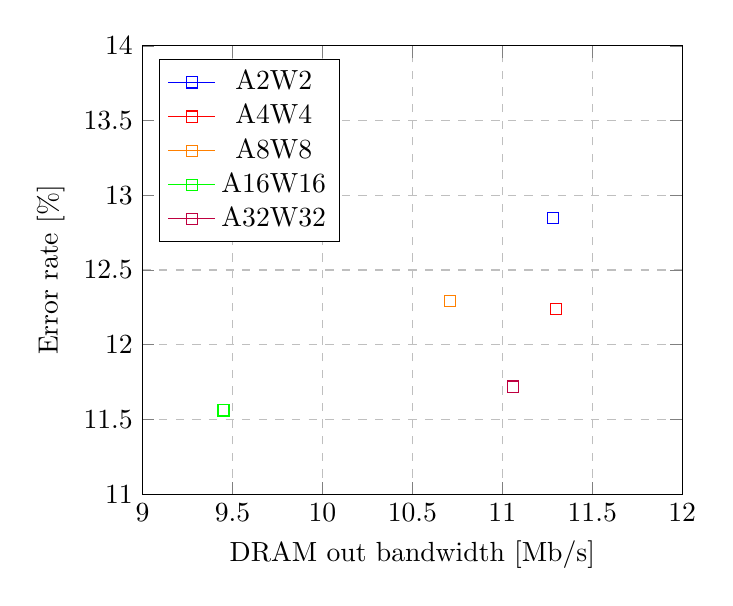
\begin{tikzpicture}
  \begin{axis}[
    xlabel={DRAM out bandwidth [Mb/s]},
    ylabel={Error rate [\%]},
    xmin=9, xmax=12,
    ymin=11, ymax=14,
    xtick={9,9.5,10,10.5,11,11.5,12},
    ytick={11,11.5,12,12.5,13,13.5,14},
    legend pos=north west,
    ymajorgrids=true,
    xmajorgrids=true,
    grid style=dashed,
    ]
  % A2W2
  \addplot+ [
      color=blue,
      mark=square
      ] coordinates {(11.28,12.85)};
  % A4W4
  \addplot+ [
      color=red,
      mark=square
      ] coordinates {(11.30,12.24)};
  % A8W8
  \addplot+ [
      color=orange,
      mark=square
      ] coordinates {(10.71,12.29)};
  % A16W16
  \addplot+ [
      color=green,
      mark=square
      ] coordinates {(9.45,11.56)};
  % A32W32
  \addplot+ [
      color=purple,
      mark=square
      ] coordinates {(11.06,11.72)};
  \legend{A2W2,A4W4,A8W8,A16W16,A32W32}
  \end{axis}
  \end{tikzpicture}
  \caption[TFC DRAM out]{TFC DRAM out bandwidth when compared to error rate}
    \label{fig:TFCDRAMOut}
  \end{figure}
\end{itemize}

%----------------------------------------------------------------------------------------
%	SUBSECTION 7.1.2 - Results Tables
%----------------------------------------------------------------------------------------

\subsection{Results Tables}

This section presents the data used to plot the different graphs from earlier but
% \begin{table}[!]
%   \centering
%   \resizebox{\textwidth}{!}{
%   \begin{tabular}{ | c | c | c | c | c | }
%     \hline
%     \textbf{Experiment Name} & \textbf{Year} &    \textbf{Paper}     & \textbf{Number of Parameters} & \textbf{Top-1 Accuracy} \\
%     \hline
%     \textbf{A2W2I8}          &     1998      &  \cite{LeCun1998}     &         0.6 M                 &           X             \\
%     \hline
%     \textbf{A4W4I8}          &     2012      & \cite{Krizhevsky2012} &          60 M                 &         63.3\%          \\
%     \hline
%     \textbf{A8W8I8}          &     2014      & \cite{Simonyan2014}   &         138 M                 &         74.4\%          \\
%     \hline
%     \textbf{A16W16I32}       &     2015      & \cite{He2015}         &          26 M                 &         81.2\%          \\
%     \hline
%     \textbf{A32W32I32}       &     2017      & \cite{Howard2017}     &         4.2 M                 &         72.56\%         \\
%     \hline
%   \end{tabular}
%   }
% \caption[Zebi]{Convolutional Neural Network Architectures}
% \label{tab:Zebi}
% \end{table}


% TFC
% Results for            Throughput | DRAM in bandwidth | DRAM out bandwidth:
% A2W2:   281951 (img/s) | 283.18 (Mb/s)     | 11.28  (Mb/s)
% A4W4:   282483 (img/s) | 289.26 (Mb/s)     | 11.30  (Mb/s)
% A8W8:   267732 (img/s) | 274.16 (Mb/s)     | 10.71  (Mb/s)
% A16W16: 236205 (img/s) | 241.87 (Mb/s)     | 9.45   (Mb/s)
% A32W32: 276541 (img/s) | 283.18 (Mb/s)     | 11.06  (MB/s)
%
% TFC
% Results for Accuracy 10 | 20 | 30 | 40 epochs
% A2W2:   84.960 | 85.540 | 86.380 | 87.150
% A4W4:   86.340 | 86.670 | 87.320 | 87.760
% A8W8:   86.010 | 87.020 | 87.460 | 87.710
% A16W16: 86.140 | 87.330 | 87.710 | 88.440
% A32W32: 86.010 | 87.340 | 87.690 | 88.280
%
% CNV
% Results for Accuracy 10 | 20 | 30 | 40 epochs
% A2W2:   65.130 | 68.710 | 76.970 | 82.360
% A4W4:   70.780 | 79.140 | 81.300 | 85.560
% A8W8:   75.450 | 81.620 | 82.760 | 85.720
% A16W16: 75.360 | 79.520 | 81.980 | 86.110
% A32W32: 72.970 | 80.760 | 82.800 | 86.050

%----------------------------------------------------------------------------------------
%	SUBSECTION 7.1.3 - Results Conclusion
%----------------------------------------------------------------------------------------

\subsection{Results Conclusion}
